\section{Experiments}
\label{sec:experiments}
\begin{table}[t]
  \centering
  \renewcommand\arraystretch{1.12}
  \setlength\tabcolsep{4pt}
  \resizebox{0.42\textwidth}{!}
{
  \begin{tabular}{cccccc}
      \noalign{\hrule height 1pt}
  &\multicolumn{1}{c}{\multirow{2}{*}{\textbf{Methods}}}   & \multicolumn{4}{c}{\textbf{RGBNT201}} \\ \cmidrule(r){3-6}
  & & \textbf{mAP} & \textbf{R-1} & \textbf{R-5} & \textbf{R-10} \\ \hline
  \multirow{14}{*}{\rotatebox{90}{\textbf{Multi-modal}}}
  & HAMNet~\cite{li2020multi}   & 27.7         & 26.3            & 41.5            & 51.7             \\
  & PFNet~\cite{zheng2021robust}    & 38.5         & 38.9            & 52.0            & 58.4             \\
  & IEEE~\cite{wang2022interact}     & 47.5         & 44.4            & 57.1            & 63.6             \\
  & DENet~\cite{zheng2023dynamic}    & 42.4         & 42.2            & 55.3            & 64.5            \\
  & LRMM~\cite{wu2025lrmm} & 52.3 & 53.4 & 64.6 & 73.2\\
  & UniCat$^*$~\cite{crawford2023unicat}   & 57.0         & 55.7            & -            & -            \\
& HTT$^*$~\cite{wang2024heterogeneous} &71.1 &73.4 &83.1 &87.3\\
& TOP-ReID$^*$~\cite{wang2024top}  &72.3 &76.6 &84.7 &89.4\\
& EDITOR$^*$~\cite{zhang2024magic} & 66.5       & 68.3           & 81.1        & 88.2             \\
& RSCNet$^*$~\cite{yu2024representation} & 68.2 & 72.5 & - & - \\
& WTSF-ReID$^*$~\cite{yu2025wtsf} & 67.9 &72.2 &83.4 &89.7 \\
& MambaPro$\dagger$~\cite{wang2024mambapro} & 78.9 & \textbf{83.4} & \underline{89.8} & 91.9 \\
& DeMo$^\dagger$~\cite{wang2024decoupled}  &\underline{79.0} 	 &\underline{82.3} 	 &88.8 	 &\underline{92.0}      \\
\rowcolor[gray]{0.92}
  & $\mathrm{\textbf{IDEA}}^\dagger$  &\textbf{80.2} 	 &82.1 	 &\textbf{90.0} 	 &\textbf{93.3}      \\
  \noalign{\hrule height 1pt}
  \end{tabular}
  }
  \vspace{-1.5mm}
  \caption{Performance comparison on RGBNT201. 
  %
  Best results are in bold, the second bests are underlined. 
  %
  $\dagger$ denotes CLIP-based methods, $*$ indicates ViT-based while others are CNN-based ones.}
  \label{tab:multi-spectral person ReID}
  \vspace{-4mm}
\end{table}
%~~~~~~~~~~~~~~~~~~~~~~~~~~~~~~~~~~~~~~~~~~~~~~~~~~~~~~~~~~~~~~~~~~~~~~~~~~~~~~~~~~~~~~~~~~~~~~~
\subsection{Datasets and Evaluation Protocols}
\textbf{Datasets.}
We evaluate the proposed method on three multi-modal object ReID benchmarks.
%
To efficiently annotate multi-spectral images without hardware constraints, we employ the API-based Qwen-VL~\cite{bai2023qwen} for automated textual description generation.
%
To be specific, RGBNT201~\cite{zheng2021robust} comprises 4,787 image triplets with 14,361 annotations, each averaging 35.47 characters and encompassing 8 distinct attributes. 
%
MSVR310~\cite{zheng2023cross} contains 2,087 image triplets and 6,261 annotations, with an average length of 56.06 characters and 6 attributes. 
%
RGBNT100~\cite{li2020multi} includes the largest number of triplets at 17,250 and 51,750 annotations with an average length of 56.25 characters and 6 attributes.
%
\\
\textbf{Evaluation Protocols.}
The performance is evaluated using mean Average Precision (mAP) and Cumulative Matching Characteristics (CMC) at Rank-K (\(K = 1, 5, 10\)). 
%
\subsection{Implementation Details}
Our model is implemented using PyTorch and trained on an NVIDIA A800 GPU. 
%
The pre-trained model CLIP~\cite{radford2021learning} is used for both the vision and text encoders. 
%
For the datasets, images triples are resized to 256$\times$128 for RGBNT201 and 128$\times$256 for MSVR310 and RGBNT100. 
%
Data augmentation includes random horizontal flipping, cropping and random erasing~\cite{zhong2020random}.
%
For RGBNT201 and MSVR310, the mini-batch size is set to 64, with 8 images sampled per identity. 
%
For RGBNT100, the mini-batch size is set to 128, with 16 images sampled per identity.
%
We fine-tune the learnable modules using an initial learning rate of 3.5$\times$10$^{-6}$, which decays to 3.5$\times$10$^{-7}$ during training.
%
For the RGBNT201 dataset, the values of \(N_{p}\) and \(k\) are set to 2 and 5, respectively.
%
Other details are provided in the supplementary material.
%
\textbf{Code and annotations are available at } \href{https://github.com/924973292/IDEA}{\textbf{IDEA}}.
\begin{table}[t]
    \centering
    \renewcommand\arraystretch{1.2}
    \setlength\tabcolsep{5pt}
    \resizebox{0.42\textwidth}{!}
	{
    \begin{tabular}{cccccc}
        \noalign{\hrule height 1pt}
    &\multicolumn{1}{c}{\multirow{2}{*}{\textbf{Methods}}} &  \multicolumn{2}{c}{\textbf{RGBNT100}} & \multicolumn{2}{c}{\textbf{MSVR310}} \\\cmidrule(r){3-4} \cmidrule(r){5-6}
    & & \textbf{mAP} & \textbf{R-1} & \textbf{mAP} & \textbf{R-1} \\
    \hline
    \multirow{18}{*}{\rotatebox{90}{\textbf{Multi-modal}}}
    &HAMNet~\cite{li2020multi} & 74.5 & 93.3 & 27.1 & 42.3 \\
    &PFNet~\cite{zheng2021robust}& 68.1 & 94.1 & 23.5 & 37.4 \\
    &GAFNet~\cite{guo2022generative} & 74.4 & 93.4 & - & - \\
    &GPFNet~\cite{he2023graph} & 75.0 & 94.5 & - & - \\
    &CCNet~\cite{zheng2023cross} & 77.2 & 96.3 & 36.4 & 55.2 \\
    & LRMM~\cite{wu2025lrmm} & 78.6 & 96.7 & 36.7 &49.7\\
    &GraFT$^*$~\cite{yin2023graft} &76.6 &94.3 &- &-\\
    &UniCat$^*$~\cite{crawford2023unicat}    & 79.4         & 96.2  & -            & -            \\
    &PHT$^*$~\cite{pan2023progressively} & 79.9 & 92.7 & - & - \\
    & HTT$^*$~\cite{wang2024heterogeneous} &75.7&92.6&- &-\\
    & TOP-ReID$^*$~\cite{wang2024top} &81.2 & 96.4 & 35.9 & 44.6 \\
    & EDITOR$^*$~\cite{zhang2024magic} & 82.1 & 96.4 &39.0 & 49.3\\
    & FACENet$^*$~\cite{zheng2025flare} & 81.5 &\underline{96.9} &36.2 &54.1 \\
    & RSCNet$^*$~\cite{yu2024representation} &82.3 &96.6 &39.5 &49.6\\
    & WTSF-ReID$^*$~\cite{yu2025wtsf} & 82.2 &96.5 & 39.2 & 49.1 \\
    & MambaPro$\dagger$~\cite{wang2024mambapro} & 83.9 & 94.7 & \underline{47.0} & 56.5 \\
    & DeMo$\dagger$~\cite{wang2024decoupled} &\underline{86.2} 	&\textbf{97.6} &\textbf{49.2}	&\underline{59.8} \\
    \rowcolor[gray]{0.92}
    & $\mathrm{\textbf{IDEA}}^\dagger$& \textbf{87.2} 	&96.5 &\underline{47.0}	&\textbf{62.4} \\
    \noalign{\hrule height 1pt}
    \end{tabular}
    }
    \vspace{-1.5mm}
    \caption{Performance on RGBNT100 and MSVR310.}
    \label{tab:multi-spectral vehicle ReID}
    \vspace{-4mm}
\end{table}
%~~~~~~~~~~~~~~~~~~~~~~~~~~~~~~~~~~~~~~~~~~~~~~~~~~~~~~~~~~~~~~~~~~~~~~~~~~~~~~~~~~~~~~~~~~~~~~~
\subsection{Comparison with State-of-the-Art Methods}
\textbf{Multi-modal Person ReID.}
In \textcolor{red}{Tab.}~\ref{tab:multi-spectral person ReID}, we compare our method IDEA$^\dagger$ with existing multi-modal approaches on the RGBNT201 dataset. 
%
Leveraging complementary information from different modalities, multi-modal methods exhibit superior performance.
%
Specifically, our proposed IDEA$^\dagger$ achieves 80.2\% mAP and 82.1\% Rank-1 accuracy, surpassing TOP-ReID$^*$ by 7.9\% in mAP and 5.5\% in Rank-1. 
%
Compared with other leading methods like HTT$^*$ and EDITOR$^*$, IDEA$^\dagger$ shows a superior adaptability to complex scenarios, confirming the robustness.
%
Besides, IDEA$^\dagger$ outperforms the CLIP-based methods MambaPro$^\dagger$ and DeMo$^\dagger$ by 1.3\% and 1.2\% in mAP, respectively.
%
These results highlight IDEA’s ability to utilize semantic information from textual guidance for improved feature discrimination. 
\\
\textbf{Multi-modal Vehicle ReID.}
In \textcolor{red}{Tab.}~\ref{tab:multi-spectral vehicle ReID}, we compare IDEA$^\dagger$ with state-of-the-art methods on the RGBNT100 and MSVR310 datasets.
%
Our IDEA$^\dagger$ achieves an mAP of 87.2\%, surpassing EDITOR$^*$ by 5.1\% in mAP.
%
Especially on the challenging MSVR310 dataset, IDEA$^\dagger$ achieves an mAP of 47.0\% and a Rank-1 accuracy of 62.4\%, outperforming EDITOR$^*$ by 8.0\% in mAP and 13.1\% in Rank-1 accuracy.
%
These results verify IDEA's generalization ability.

%~~~~~~~~~~~~~~~~~~~~~~~~~~~~~~~~~~~~~~~~~~~~~~~~~~~~~~~~~~~~~~~~~~~~~~~~~~~~~~~~~~~~~~~~~~~~~~~
\begin{table}[t]
  \centering
  \renewcommand\arraystretch{1.0}
  \setlength\tabcolsep{4.5pt}
  \resizebox{0.35\textwidth}{!}
  {
  \begin{tabular}{cccccc}
      \noalign{\hrule height 1pt}
      \multicolumn{1}{c}{\multirow{2}{*}{\textbf{Index}}} &\multicolumn{3}{c}{\textbf{Modules}} & \multicolumn{2}{c}{\textbf{Metrics}} \\
      \cmidrule(r){2-4} \cmidrule(r){5-6}
 & \textbf{Text}              & \textbf{IMFE}                & \textbf{CDA}                   & \textbf{mAP}    & \textbf{Rank-1}   \\\hline
  A                  & \ding{53}                  & \ding{53}                  & \ding{53}                    & 70.3  & 72.1 \\
  B                  & \ding{51}                  & \ding{53}                  & \ding{53}                      & 73.4  & 75.8 \\
  \multirow{1}{*}{C} & \multirow{1}{*}{\ding{51}} & \multirow{1}{*}{\ding{51}} & \multirow{1}{*}{\ding{53}}    & 77.2  & 81.1 \\
  \rowcolor[gray]{0.92}
  \multirow{1}{*}{D} & \multirow{1}{*}{\ding{51}} & \multirow{1}{*}{\ding{51}} & \multirow{1}{*}{\ding{51}}    &\textbf{80.2} &\textbf{82.1}  \\
  \noalign{\hrule height 1pt}
  \end{tabular}
  }
  \vspace{-1.5mm}
  \caption{Performance comparison with different modules.}
  \label{tab:main_ablation}
  \vspace{-2mm}
\end{table}
%~~~~~~~~~~~~~~~~~~~~~~~~~~~~~~~~~~~~~~~~~~~~~~~~~~~~~~~~~~~~~~~~~~~~~~~~~~~~~~~~~~~~~~~~~~~~~~~
\begin{table}[t]
  \centering
  \renewcommand\arraystretch{1.0}
  \setlength\tabcolsep{4.5pt}
  \resizebox{0.42\textwidth}{!}
  {
  \begin{tabular}{cccccc}
      \noalign{\hrule height 1pt}
      \multicolumn{1}{c}{\multirow{2}{*}{\textbf{Index}}} &\multicolumn{3}{c}{\textbf{IMFE}} & \multicolumn{2}{c}{\textbf{Metrics}} \\
      \cmidrule(r){2-4} \cmidrule(r){5-6}
 & \textbf{InverseNet}              & \textbf{Prefixes}                & \textbf{Prompt}                   & \textbf{mAP}    & \textbf{Rank-1}   \\\hline
  A                   & \ding{53}                  & \ding{53}                 & -                     & 72.6 & 75.1  \\
  B                  & \ding{53}                  & \ding{51}                  & \ding{53}                     & 73.4  & 75.8                   \\
  C                  & \ding{51}                  & \ding{53}                  & -                    & 73.7  & 77.3                   \\
  D                  & \ding{51}                  & \ding{51}                  & \ding{53}                      & 75.4  & 78.6               \\
  \rowcolor[gray]{0.92}
  E & \multirow{1}{*}{\ding{51}} & \multirow{1}{*}{\ding{51}} & \multirow{1}{*}{\ding{51}}    & \textbf{77.2}  & \textbf{81.1}  \\
  \noalign{\hrule height 1pt}
  \end{tabular}
  }
  \vspace{-1.5mm}
  \caption{Comparison with different components in IMFE.}
  \label{tab:IMFE_ablation}
  \vspace{-4mm}
\end{table}
%~~~~~~~~~~~~~~~~~~~~~~~~~~~~~~~~~~~~~~~~~~~~~~~~~~~~~~~~~~~~~~~~~~~~~~~~~~~~~~~~~~~~~~~~~~~~~~~
\subsection{Ablation Studies}
We evaluate the effectiveness of the proposed modules on the RGBNT201 dataset. 
%
To be specific, our baseline comprises a three-branch vision encoder, which performs retrieval by concatenating the class tokens from three modalities. 
%
Upon incorporating the IMFE, we utilize \( F^{t}_{G} \) for retrieval and when the CDA is included, \( F^{t}_{CDA} \) is employed.
\\
\textbf{Effects of Key Modules.}
\textcolor{red}{Tab.}~\ref{tab:main_ablation} presents the performance of various combinations of our proposed modules. 
%
Model A serves as the baseline, achieving an mAP of 70.3\% and Rank-1 accuracy of 72.1\%.
%
Model B incorporates text information through parallel text encoders, improving the mAP to 73.4\% and Rank-1 accuracy to 75.8\%. 
%
With the inverted structure in IMFE, Model C further enhances performance, reaching an mAP of 77.2\% and Rank-1 of 81.1\%. 
%
Finally, Model D integrates CDA, delivering the best performance with an mAP of 80.2\%.
%
These results fully validate the effectiveness and efficiency of the proposed modules.
%~~~~~~~~~~~~~~~~~~~~~~~~~~~~~~~~~~~~~~~~~~~~~~~~~~~~~~~~~~~~~~~~~~~~~~~~~~~~~~~~~~~~~~~~~~~~~~~
\begin{table}[t]
  \centering
  \renewcommand\arraystretch{1.0}
  \setlength\tabcolsep{4.5pt}
  \resizebox{0.42\textwidth}{!}
  {
  \begin{tabular}{cccccc}
      \noalign{\hrule height 1pt}
      \multicolumn{1}{c}{\multirow{2}{*}{\textbf{Index}}} &\multicolumn{3}{c}{\textbf{CDA}} & \multicolumn{2}{c}{\textbf{Metrics}} \\
      \cmidrule(r){2-4} \cmidrule(r){5-6}
& \textbf{Sample}              & \textbf{Cross Attn}                & \textbf{Shared Offset}                   & \textbf{mAP}    & \textbf{Rank-1}   \\\hline
A                   & \ding{53}                  & \ding{53}                  & - & 76.3  & 78.7   \\
B                  & \ding{53}                  & \ding{51}                  & -                     & 77.0  & 79.8                    \\
C                  & \ding{51}                  & \ding{53}                  & \ding{53}                    & 76.8  & 78.9                    \\
D                  & \ding{51}                  & \ding{53}                  & \ding{51}                      & 77.6  & 80.4                \\
E                  & \ding{51}                  & \ding{51}                  & \ding{53}                      & 79.5  & 81.7                \\
\rowcolor[gray]{0.92}
F & \multirow{1}{*}{\ding{51}} & \multirow{1}{*}{\ding{51}} & \multirow{1}{*}{\ding{51}}     &\textbf{80.2}  &\textbf{82.1}   \\
  \noalign{\hrule height 1pt}
  \end{tabular}
  }
  \vspace{-1.5mm}
  \caption{Comparison with different components in CDA.}
  \label{tab:CDA_ablation}
  \vspace{-3mm}
\end{table}
%~~~~~~~~~~~~~~~~~~~~~~~~~~~~~~~~~~~~~~~~~~~~~~~~~~~~~~~~~~~~~~~~~~~~~~~~~~~~~~~~~~~~~~~~~~~~~~~
\begin{table}[t]
  \centering
  \renewcommand\arraystretch{1.0}
  \setlength\tabcolsep{4.5pt}
  \resizebox{0.42\textwidth}{!}
  {
  \begin{tabular}{cccccc}
      \noalign{\hrule height 1pt}
      \multicolumn{1}{c}{\textbf{Model}} & \textbf{mAP} & \textbf{Rank-1} & \textbf{Rank-5} & \textbf{Rank-10} \\ \hline
  IDEA w/o Text  & 74.5 & 75.0 & 84.8 & 88.8 \\
  \rowcolor[gray]{0.92}
  IDEA            & \textbf{80.2} & \textbf{82.1} & \textbf{90.0} & \textbf{93.3} \\
      \noalign{\hrule height 1pt}
  \end{tabular}
  }
  \vspace{-1.5mm}
  \caption{Comparison of IDEA with and without text.}
  \label{tab:Text_ablation}
  \vspace{-3mm}
\end{table}
%~~~~~~~~~~~~~~~~~~~~~~~~~~~~~~~~~~~~~~~~~~~~~~~~~~~~~~~~~~~~~~~~~~~~~~~~~~~~~~~~~~~~~~~~~~~~~~~
\begin{table}[t]
  \centering
  \renewcommand\arraystretch{1.0}
  \setlength\tabcolsep{4.5pt}
  \resizebox{0.42\textwidth}{!}
  {
  \begin{tabular}{cccccccc}
      \noalign{\hrule height 1pt}
      \multicolumn{1}{c}{\textbf{Model}} & \textbf{mAP} & \textbf{Rank-1} & \textbf{Rank-5} & \textbf{Rank-10} \\ \hline
  IDEA w/o Offset  & 78.4 & 81.3 & 89.7 & 92.2 \\
  \rowcolor[gray]{0.92}
  IDEA            & \textbf{80.2} & \textbf{82.1} & \textbf{90.0} & \textbf{93.3} \\
      \noalign{\hrule height 1pt}
  \end{tabular}
  }
  \vspace{-1.5mm}
  \caption{Comparison of IDEA with and without offset.}
  \label{tab:Offset_ablation}
  \vspace{-3mm}
\end{table}
%~~~~~~~~~~~~~~~~~~~~~~~~~~~~~~~~~~~~~~~~~~~~~~~~~~~~~~~~~~~~~~~~~~~~~~~~~~~~~~~~~~~~~~~~~~~~~~~
\\
\textbf{Effects of Key Components in IMFE.}
\textcolor{red}{Tab.}~\ref{tab:IMFE_ablation} shows the performance of different components in the IMFE.
%
Model A represents the parallel text encoders without the inverted structure or prefixes, achieving an mAP of 72.6\% and Rank-1 accuracy of 75.1\%.
%
With the Modal Prefixes in Model B, the mAP increases to 73.4\%, demonstrating the effectiveness of our prefixes mechanism.
%
Model C introduces the inverted structure, achieving an mAP of 73.7\%.
%
Model D combines the inverted structure and prefixes, further improving the mAP to 75.4\%.
%
Finally, Model E integrates the learnable tokens in Modal Prefixes, achieving the best performance with an mAP of 77.2\%.
%
Overall, inverted structure performs better than the parallel structure, achieving better performance.
%
These results demonstrate the effectiveness of different components in our proposed IMFE.
\\
\textbf{Effects of Key Components in CDA.}
Based on the IMFE, \textcolor{red}{Tab.}~\ref{tab:CDA_ablation} shows the performance of various components within CDA.
%
When sampling is excluded, all local patches in \( \hat{F}_{m} \) are processed.
%
Without cross attention, multi-modal interaction uses only local features, omitting global context, with pooled \( \hat{F}_{m} \) for retrieval.
%
If shared offset is excluded, each modality independently generates offsets.
%
Regarding numerical results, Model A, which does not incorporate these components, achieves an mAP of 76.3\% and Rank-1 accuracy of 78.7\%.
%
Model B introduces cross attention, leading to a slight improvement in mAP to 77.0\%.
%
Model C adds sampling, resulting in a 0.5\% improvement in mAP over Model A by reducing noise in the local features.
%
Model D incorporates shared offset, yielding a 0.8\% improvement in mAP and a 1.5\% increase in Rank-1 accuracy compared to Model C.
%
Model E combines cross attention and sampling, achieving an mAP of 79.5\%.
%
Finally, Model F delivers the best performance with an mAP of 80.2\%.
%
These results validate the effectiveness of each component within CDA.
\\
\textbf{Effects of Text Guidance in IDEA.}
\textcolor{red}{Tab.}~\ref{tab:Text_ablation} compares IDEA's performance with and without text input.
%
Model A, lacking text input, achieves an mAP of 74.5\%. 
%
With text guidance, Model B improves to 80.2\% mAP, demonstrating the effectiveness of text in enhancing feature robustness.
%
\\
\textbf{Effects of Offset in IDEA.}
\textcolor{red}{Tab.}~\ref{tab:Offset_ablation} compares the performance of IDEA with and without the offset mechanism.
%
Model A uses aggregated local features with convolution to interact with global features, achieving an mAP of 78.4\% and Rank-1 accuracy of 81.3\%.
%
Model B introduces the offset mechanism, improving the mAP to 80.2\% and Rank-1 accuracy to 82.1\%. 
%
This demonstrates that the offset mechanism helps the model focus on more important regions.
\\
\textbf{Effects of Prompt Lengths and Offset Factors.}
\textcolor{red}{Fig.}~\ref{fig:hyper} illustrates the performance of IDEA with varying prompt lengths and offset factors. 
%
The results show that a prompt length of 2 and an offset factor of 5 yield the best performance.
%
As the prompt length increases, the model's performance improves, but the gains become smaller as the prompt length grows, likely due to the text truncation.
%
Regarding the offset factor, the model remains stable.
%~~~~~~~~~~~~~~~~~~~~~~~~~~~~~~~~~~~~~~~~~~~~~~~~~~~~~~~~~~~~~~~~~~~~~~~~~~~~~~~~~~~~~~~~~~~~~~~
\begin{figure}[t]
  \centering
    \resizebox{0.475\textwidth}{!}
    {
  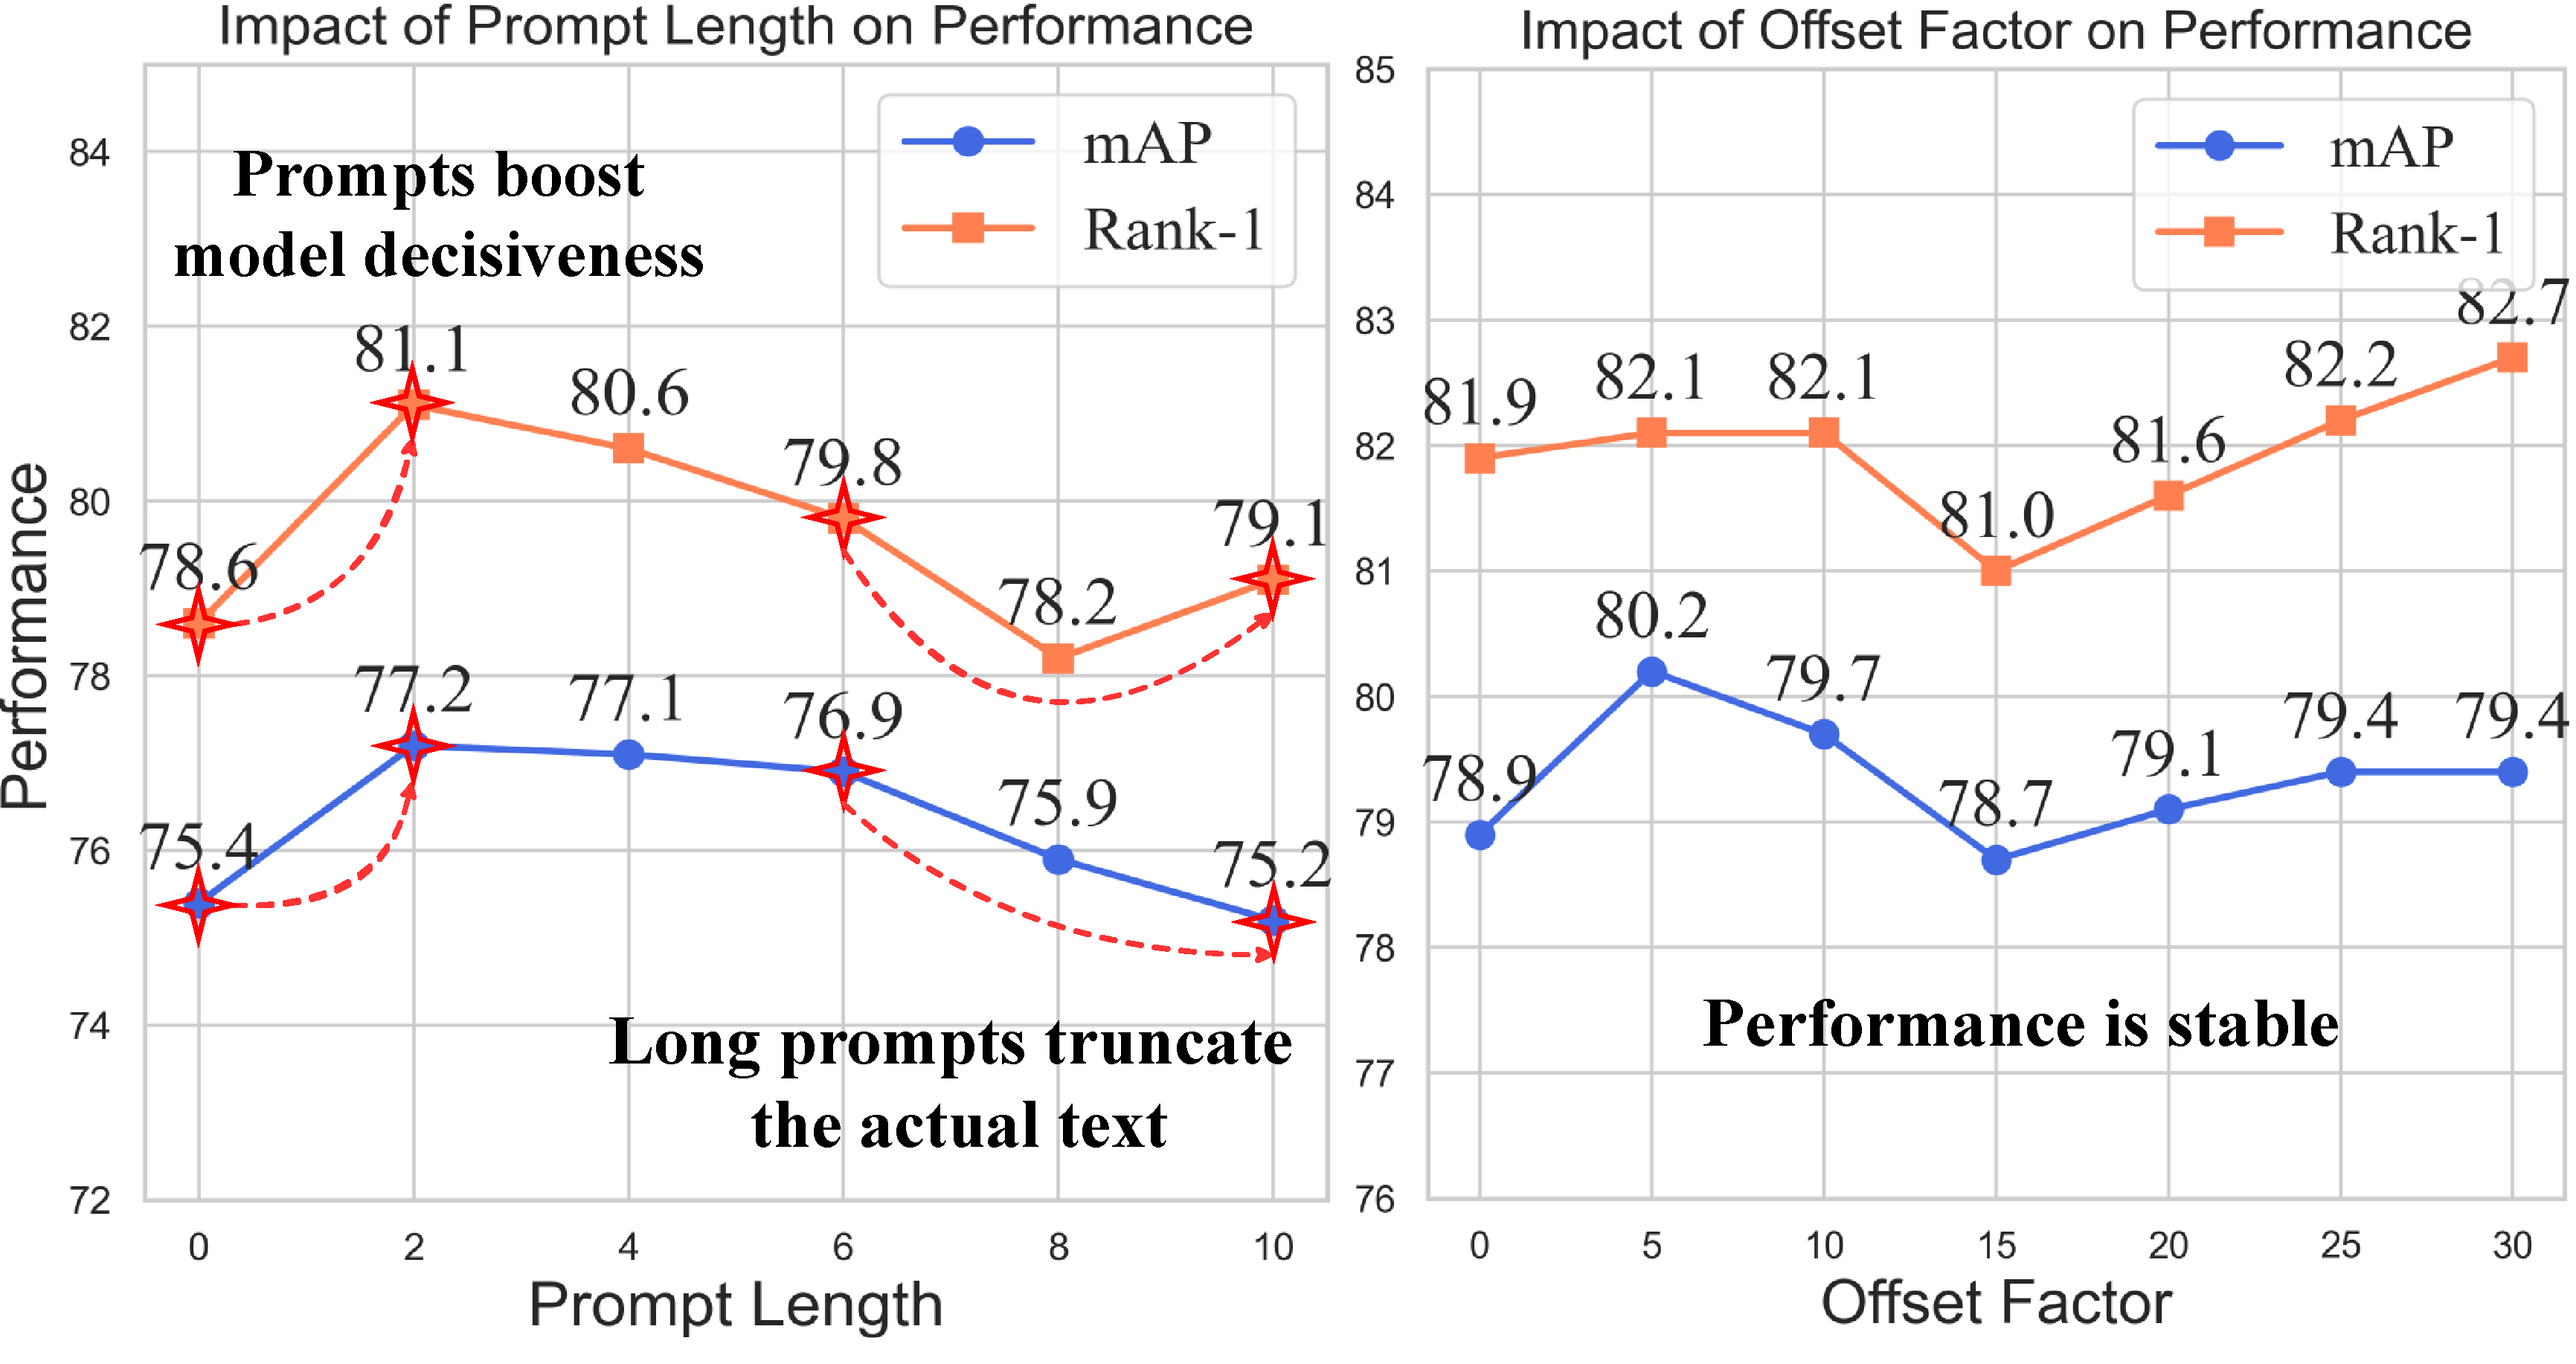
\includegraphics[width=1.\linewidth]{sec/img/Hyper.pdf}
  }
  \vspace{-5mm}
   \caption{Comparison with different hyper-parameters.}
  \label{fig:hyper}
  \vspace{-2mm}
\end{figure}
%~~~~~~~~~~~~~~~~~~~~~~~~~~~~~~~~~~~~~~~~~~~~~~~~~~~~~~~~~~~~~~~~~~~~~~~~~~~~~~~~~~~~~~~~~~~~~~~
\begin{figure}[t]
  \centering
    \resizebox{0.475\textwidth}{!}
    {
  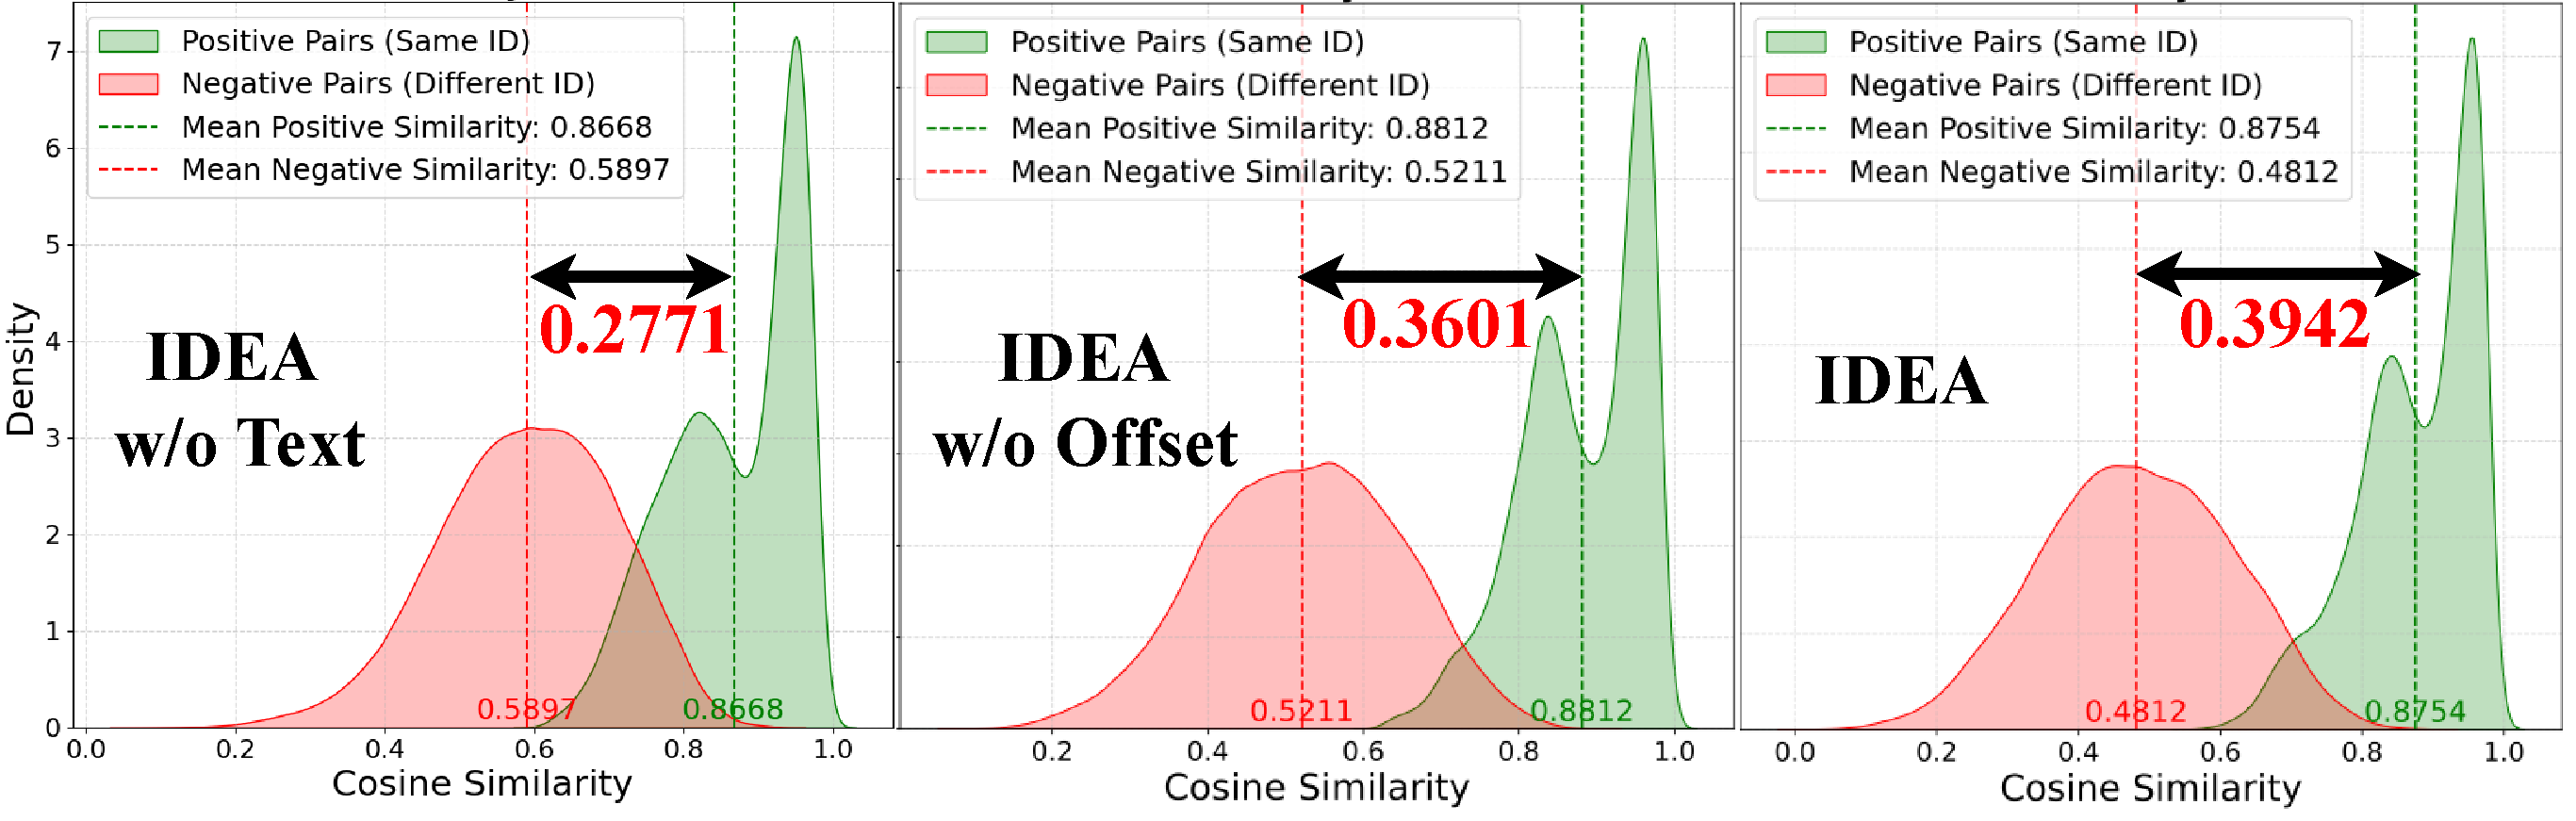
\includegraphics[width=30.\linewidth]{sec/img/CosDis.pdf}
  }
  \vspace{-5mm}
   \caption{Visualization of the cosine similarity distribution.}
  \label{fig:cosine}
  \vspace{-4mm}
\end{figure}
%~~~~~~~~~~~~~~~~~~~~~~~~~~~~~~~~~~~~~~~~~~~~~~~~~~~~~~~~~~~~~~~~~~~~~~~~~~~~~~~~~~~~~~~~~~~~~~~
\begin{figure*}[t]
  \centering
    \resizebox{0.96\textwidth}{!}
    {
  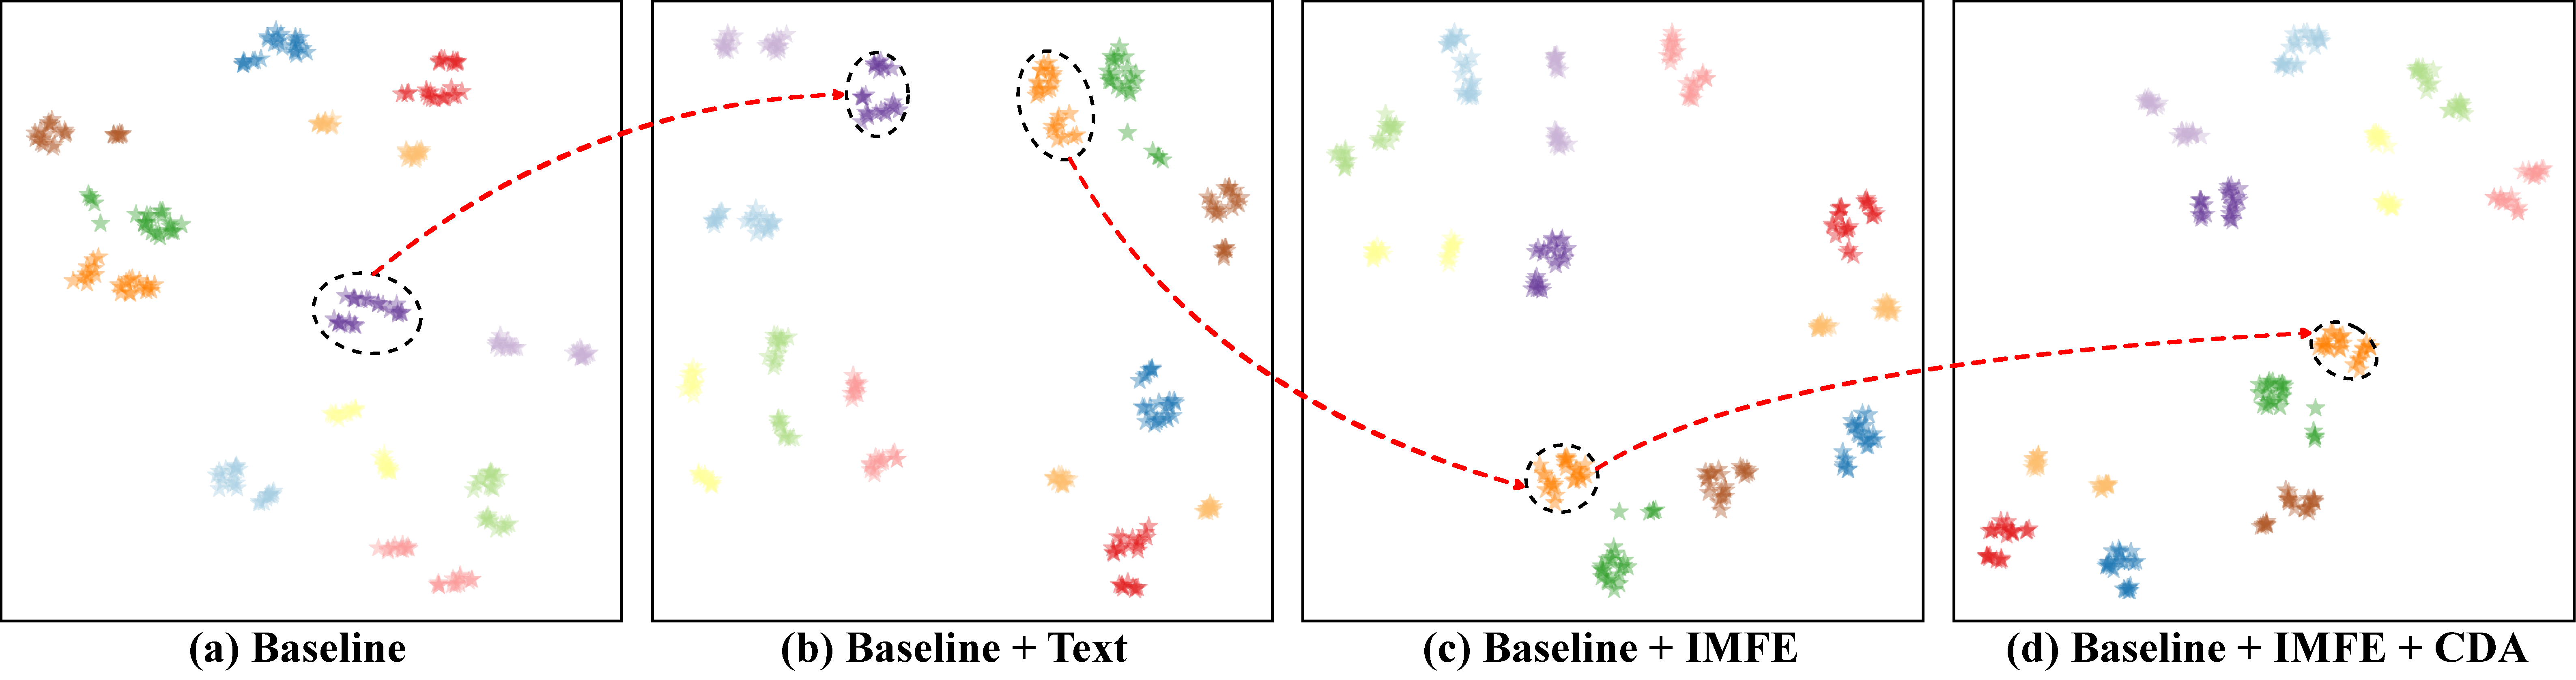
\includegraphics[width=1\linewidth]{sec/img/tsne.pdf}
  }
  \vspace{-2mm}
   \caption{Visualization of the feature distributions with t-SNE~\cite{van2008visualizing}.
   %
   Different colors represent different identities.}
  \label{fig:tsne}
  \vspace{-5mm}
\end{figure*}
%~~~~~~~~~~~~~~~~~~~~~~~~~~~~~~~~~~~~~~~~~~~~~~~~~~~~~~~~~~~~~~~~~~~~~~~~~~~~~~~~~~~~~~~~~~~~~~~
\begin{figure}[t]
  \centering
    \resizebox{0.45\textwidth}{!}
    {
  \includegraphics[width=1.\linewidth]{sec/img/off_set.pdf}
  }
  \vspace{-2mm}
   \caption{Visualization of the generated offsets.}
  \label{fig:off_set}
  \vspace{-4mm}
\end{figure}
%~~~~~~~~~~~~~~~~~~~~~~~~~~~~~~~~~~~~~~~~~~~~~~~~~~~~~~~~~~~~~~~~~~~~~~~~~~~~~~~~~~~~~~~~~~~~~~~
\begin{figure}[t]
  \centering
    \resizebox{0.45\textwidth}{!}
    {
  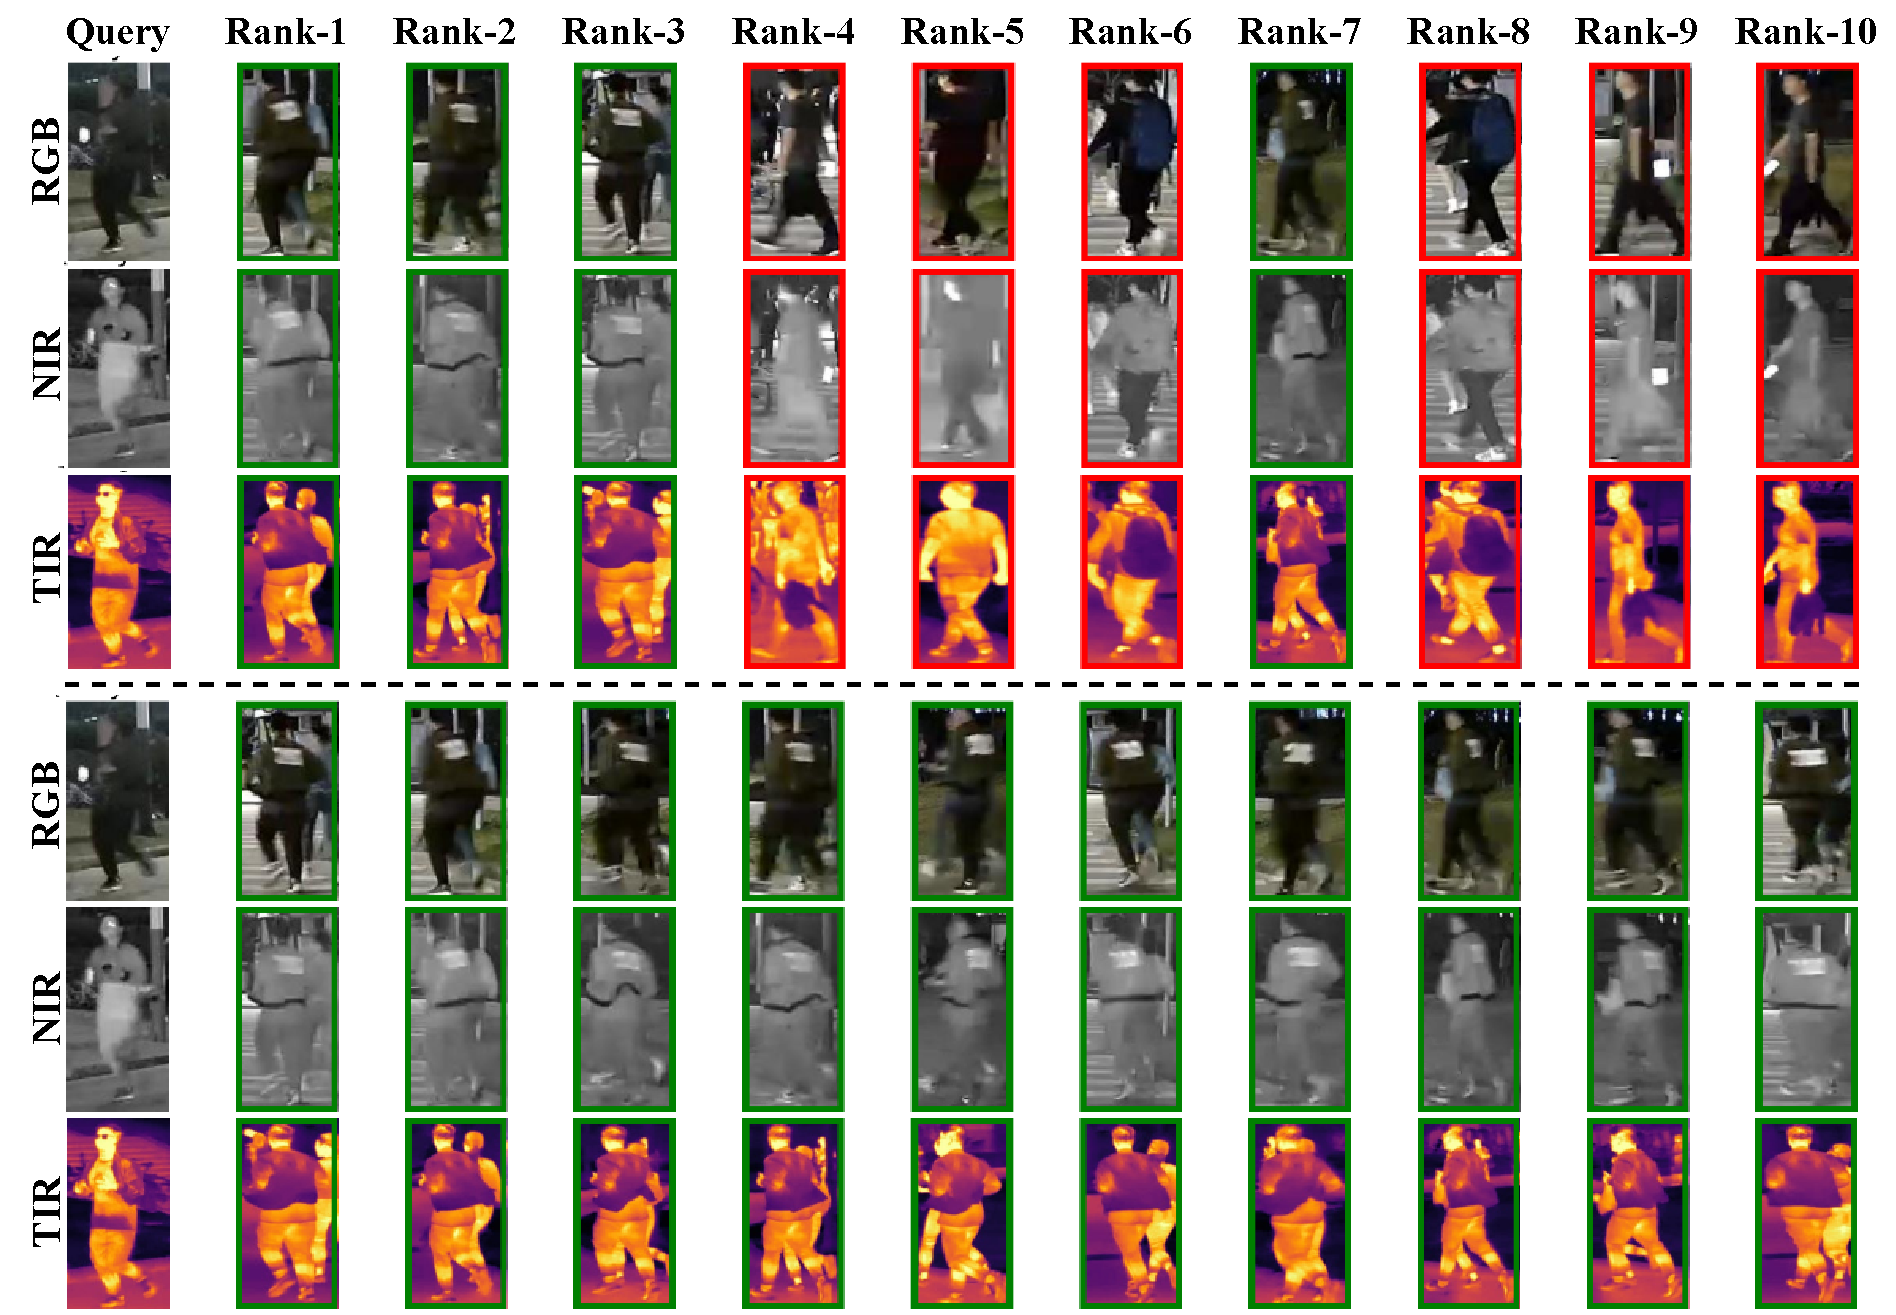
\includegraphics[width=30\linewidth]{sec/img/rank-list.pdf}
  }
  \vspace{-2mm}
   \caption{Rank list comparison between the baseline and IDEA.}
  \label{fig:rank_list}
  \vspace{-5mm}
\end{figure}
%~~~~~~~~~~~~~~~~~~~~~~~~~~~~~~~~~~~~~~~~~~~~~~~~~~~~~~~~~~~~~~~~~~~~~~~~~~~~~~~~~~~~~~~~~~~~~~~
\begin{figure}[t]
  \centering
    \resizebox{0.45\textwidth}{!}
    {
  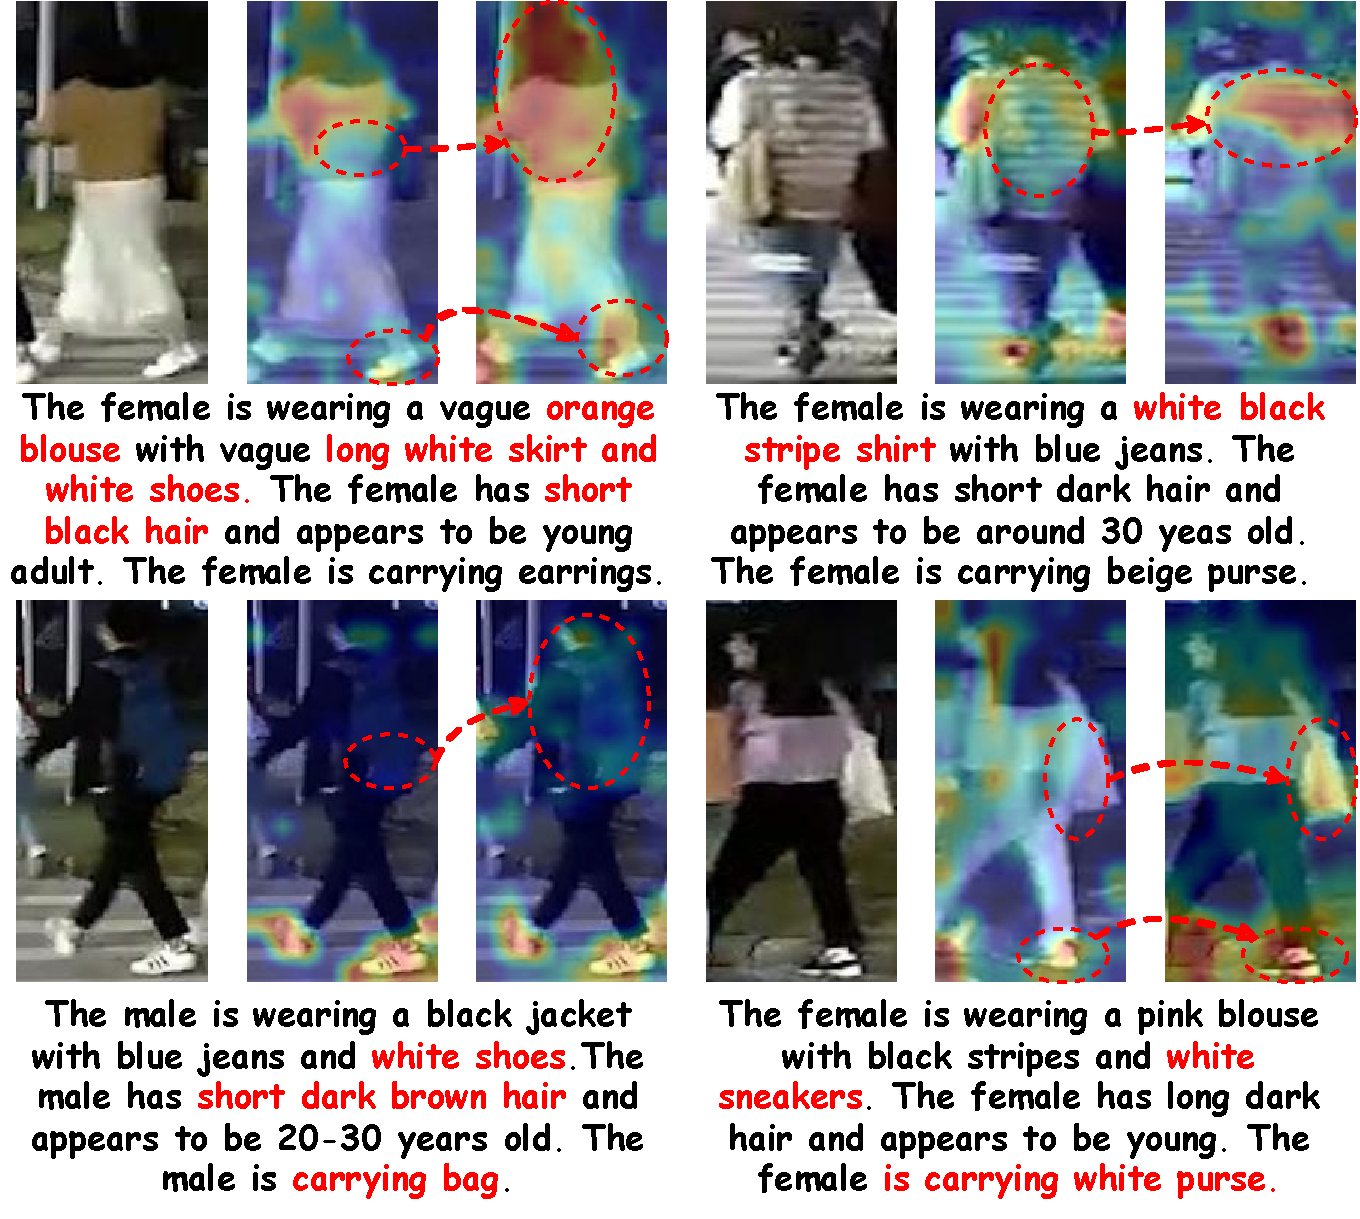
\includegraphics[width=30\linewidth]{sec/img/ChannelAct.pdf}
  }
  \vspace{-1mm}
   \caption{Visualization of the channel activation maps.
   %
   Each set includes the original image, baseline and IDEA map, respectively.}
  \label{fig:text_gain}
  \vspace{-5mm}
\end{figure}
\subsection{Visualization Analysis}
\textbf{Cosine Similarity Distributions.}
\textcolor{red}{Fig.}~\ref{fig:cosine} presents the distributions of cosine similarities among test features.
%
The results verify that incorporating text enhances feature discrimination, while adding offset mechanism further amplifies the distinction between positive and negative samples, confirming the capture of more discriminative features.
\\
\textbf{Multi-modal Feature Distributions.}
\textcolor{red}{Fig.}~\ref{fig:tsne} visualizes the feature distributions of different modules.
%
Comparing \textcolor{red}{Fig.}~\ref{fig:tsne} (a) and (b), the introduction with text guidance improves feature discrimination, as instances of the same ID become more compact.
%
In \textcolor{red}{Fig.}~\ref{fig:tsne} (c), with IMFE, the feature distributions become more discriminative than the parallel structure in \textcolor{red}{Fig.}~\ref{fig:tsne} (b).
%
Finally, in \textcolor{red}{Fig.}~\ref{fig:tsne} (d), CDA further enhances feature discrimination.
%
These visualizations demonstrate the effectiveness of our proposed modules.
%
\\
\textbf{Visualization of the Generated Offsets.}
\textcolor{red}{Fig.}~\ref{fig:off_set} visualizes the offsets generated by CDA.
%
Each arrow starts at the reference point and ends at the feature sampling point.
%
We map these offsets onto the original image to identify the regions where the model shifts its attention.
%
As shown, the offsets highlight discriminative areas, such as the head, bag and shoes. 
%
It demonstrates how the offset mechanism guides the model to focus on the most discriminative regions, effectively reducing the influence of noisy information.
\\
\textbf{Rank List Comparison.}
\textcolor{red}{Fig.}~\ref{fig:rank_list} compares the cross-camera rank lists from the baseline and IDEA.
%
IDEA produces more accurate rankings, while the baseline yields noisier results.
%
These visualizations validate the effectiveness of IDEA.
\\
\textbf{Visualization of Channel Activation Maps.}
\textcolor{red}{Fig.}~\ref{fig:text_gain} compares the channel activation maps of our baseline model and IDEA.
%
The incorporation of textual guidance helps the model focus on more discriminative regions, enhancing feature robustness and improving interpretability.



